%\chapter*{附錄：何時被提}
%\phantomsection
%\addcontentsline{toc}{chapter}{附錄：何時被提}
%\markboth{附錄：何時被提}{附錄：何時被提}
%\setcounter{figure}{0}
%\renewcommand{\thefigure}{\arabic{figure}}   % this is the line that fixes \ref
%\def\theHfigure{appendix.\arabic{figure}}



%\appendix
\renewcommand{\appendixname}{附錄}
\renewcommand{\thechapter}{\arabic{chapter}}
\renewcommand{\thefigure}{\appendixname~\thechapter.\arabic{figure}}  % Appendix 1.1, 1.2, …

\refstepcounter{chapter}
\chapter*{附錄：何時被提}
\addcontentsline{toc}{chapter}%
  {\appendixname~\thechapter\quad 何時被提？}



\section*{什麼是「被提」（Rapture）？}


「被提」（Rapture）是指耶穌基督再來時，信徒被提到主那裡，與主相遇。主要根據是帖撒羅尼迦前書4:13–18，以及哥林多前書15:51–52等經文。

\begin{quote}

「論到睡了的人、我們不願意弟兄們不知道、恐怕你們憂傷、像那些沒有指望的人一樣。
我們若信耶穌死而復活了、那已經在耶穌裡睡了的人、　神也必將他與耶穌一同帶來。
我們現在照主的話告訴你們一件事．我們這活著還存留到主降臨的人、斷不能在那已經睡了的人之先．
因為主必親自從天降臨、有呼叫的聲音、和天使長的聲音、又有　神的號吹響．那在基督裡死了的人必先復活。
以後我們這活著還存留的人、必和他們一同被提到雲裡、在空中與主相遇．這樣、我們就要和主永遠同在。
所以你們當用這些話彼此勸慰。」（帖撒羅尼迦前書4:13–18）
\end{quote}

\begin{quote}
「我如今把一件奧秘的事告訴你們．我們不是都要睡覺、乃是都要改變。
就在一霎時、眨眼之間、號筒末次吹響的時候．因號筒要響、死人要復活成為不朽壞的、我們也要改變。」（哥林多前書15:51–52）
\end{quote}

被提可以分為「災前」、「災中」、「災後」被提三種。新約並沒有一節經文直接說「大災難之前被提」。以下的解釋是解經家根據經文的推論。

\section*{災前被提（Pretribulation）}

因為新約多處應許信徒必蒙保守，脫離將來神的忿怒。災前被提的觀點認為，教會要在七年大災難開始之前被提。主要依據的經文如下：

\begin{itemize}
\item 帖撒羅尼迦前書1:10：「救我們脫離將來忿怒的耶穌。」
\item 帖撒羅尼迦前書5:9：「神不是預定我們受刑、乃是預定我們藉著我們主耶穌基督得救。」這裡的「刑」原文就是「忿怒」，而上下文（5:1–3）講的正是主的日子。
\item 羅馬書5:9：「我們……更要藉著他免去神的忿怒。」
\item 啟示錄3:10：「我必在普天下人受試煉的時候、保守你免去你的試煉。」「免去」原文是「保守脫離」，意思是不在那段時間之中，而不只是在其中被保守。
\item 路加福音21:36：「你們要時時警醒、常常祈求、使你們能逃避這一切要來的事、得以站立在人子面前。」
\end{itemize}

另外，在舊約也有許多的預表：
\begin{itemize}
\item 創世記5:24：以諾在洪水審判之前被神取去。
\item 創世記19:22：天使對羅得說：「你要速速的逃到那城、因為你還沒有到那裡、我不能作甚麼。」審判要等義人離開以後才會降下。
\end{itemize}

如圖\ref{fig:pretribulation}所示：\ding{172}教會時期、\ding{173}大患難前被提、\ding{174}與耶穌一同回到地面作王、\ding{175}大災難、\ding{176}千禧年、\ding{177}新天新地。
    
\begin{figure}[htbp]
    \centering
    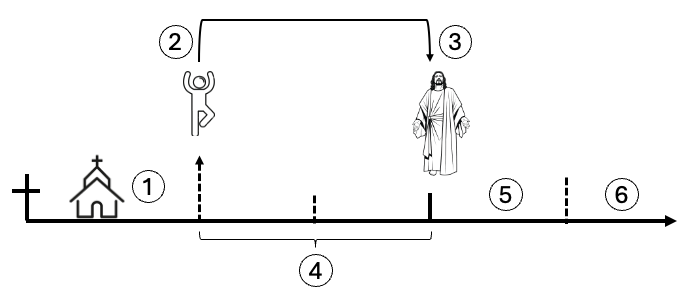
\includegraphics[
    width=1\textwidth, 
    trim=0 0 0 0, 
    clip]{images/pretribulation.png}
    \caption{災前被提}
    \label{fig:pretribulation}
\end{figure}




\section*{災中被提（Midtribulation）}

災中被提的觀點認為，教會要經過大災難的前三年半，在「一七之半」、神的忿怒傾倒之前被提，因為聖經把七年的中間點標示為轉折，而「末次的號筒」正在那時吹響：

\begin{itemize}
\item 但以理書9:27：「一七之半、他必使祭祀與供獻止息。」七年的中間點是整段時期的分水嶺。
\item 哥林多前書15:52：「號筒末次吹響的時候……我們也要改變。」災中被提派認為這「末次的號筒」就是啟示錄11:15的第七號。
\item 啟示錄11:11-12：兩個見證人傳道一千二百六十天（三年半）以後，聽見天上有聲音說：「上到這裡來。」他們就駕著雲上了天。這被視為信徒在災中被提的圖畫。
\item 啟示錄11:15、18：第七位天使吹號，天上說：「你的忿怒臨到了。」神的忿怒（七碗之災，啟16章）在後半段才傾倒。
\item 帖撒羅尼迦前書5:9：「神不是預定我們受刑」（原文「忿怒」）。災中被提派認為，前三年半是人和敵基督的逼迫，後三年半才是神的忿怒，信徒要在神的忿怒臨到之前被提。
\item 帖撒羅尼迦後書2:3-4：信徒被聚集之前，那大罪人要先「坐在神的殿裡、自稱是神」。這正是發生在七年中間的事（太24:15）。
\end{itemize}

如圖\ref{fig:midtribulation}所示：\ding{172}教會時期、\ding{173}大患難中被提、\ding{174}與耶穌一同回到地面作王、\ding{175}大災難、\ding{176}千禧年、\ding{177}新天新地。
\begin{figure}[htbp]
    \centering
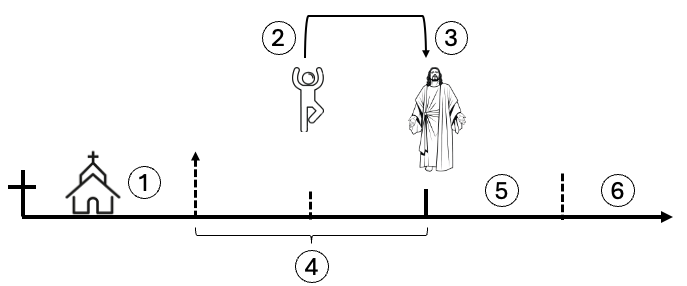
\includegraphics[
    width=1\textwidth, 
    trim=0 0 0 0, 
    clip]{images/midtribulation.png}
    \caption{災中被提}
    \label{fig:midtribulation}
\end{figure}

\section*{災後被提（Posttribulation）}

災後被提的觀點認為，教會要經過大災難，到災難結束、基督在榮耀中再來的時候，信徒才被提到空中與主相遇，因為新約描寫的「聚集選民」都在大災難之後：

\begin{itemize}
\item 馬太福音24:29-31：「那些日子的災難一過去……他要差遣使者、用號筒的大聲、將他的選民、從四方……都招聚了來。」主明說聚集選民是在災難之後。
\item 帖撒羅尼迦後書2:1-3：「論到我們主耶穌基督降臨、和我們到他那裡聚集……因為那日子以前、必有離道反教的事、並有那大罪人……顯露出來。」保羅說信徒被聚集之前，敵基督要先出現。
\item 帖撒羅尼迦後書1:6-7：「你們這受患難的人、與我們同得平安、那時主耶穌同他有能力的天使、從天上在火焰中顯現。」信徒得安息是在主公開顯現的時候。
\item 哥林多前書15:52：「號筒末次吹響的時候」，與馬太福音24:31的號筒，被認為是同一個時刻。
\item 啟示錄20:4-5：為耶穌作見證、沒有拜獸的人都復活了，「這是頭一次的復活」。如果「頭一次的復活」在大災難之後，信徒的復活和被提就也在災後。
\item 約翰福音17:15：「我不求你叫他們離開世界、只求你保守他們脫離那惡者。」神保守信徒的方式是在患難中保守，而不是把他們帶離患難。
\end{itemize}

另外，在舊約也有許多的預表：
\begin{itemize}
\item 創世記7:1、23：挪亞沒有在洪水以前被取去，而是在方舟裡經過洪水，蒙神保守。
\item 出埃及記8:22：神降災的時候，以色列人仍住在埃及，但神把歌珊地分別出來，災禍沒有臨到他們。
\end{itemize}

如圖\ref{fig:posttribulation}所示：\ding{172}教會時期、\ding{173}大患難後被提、\ding{174}與耶穌一同回到地面作王、\ding{175}大災難、\ding{176}千禧年、\ding{177}新天新地）。
\begin{figure}[htbp]
    \centering
    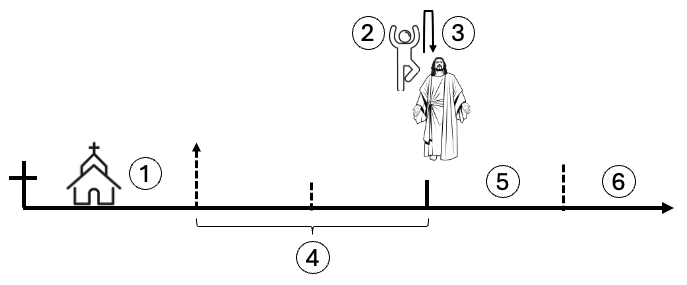
\includegraphics[
    width=1\textwidth, 
    trim=0 0 0 0, 
    clip]{images/posttribulation.png}
    \caption{災後被提}
    \label{fig:posttribulation}
\end{figure}


